\chapter{Besonderheiten}
\section{Mobile Version}

\FloatBarrier

Im Lastenheft wurde erwähnt, dass es in einer zweiten Ausbaustufe möglich sein soll, Aufgaben auf mobilen Geräten einzusehen und abhaken zu können. Dafür wurde geplant, dass diese mobile Version über eine Schnittstelle mit dem hier entworfenen System kommuniziert und als Mobile-App auf den mobilen Geräten zur Verfügung steht.

Dafür wurden im Entwurf die einzelnen Endpunkte der REST-Schnittstelle spezifiziert und ausdefiniert, über welche die mobile Anwendung alle nötigen Daten senden und empfangen kann. Diese Schnittstelle ist möglichst minimal gehalten, um keine Funktionalität zu implementieren, die nicht weiter benötigt wird.

\begin{figure}[ht!]
    \centering
    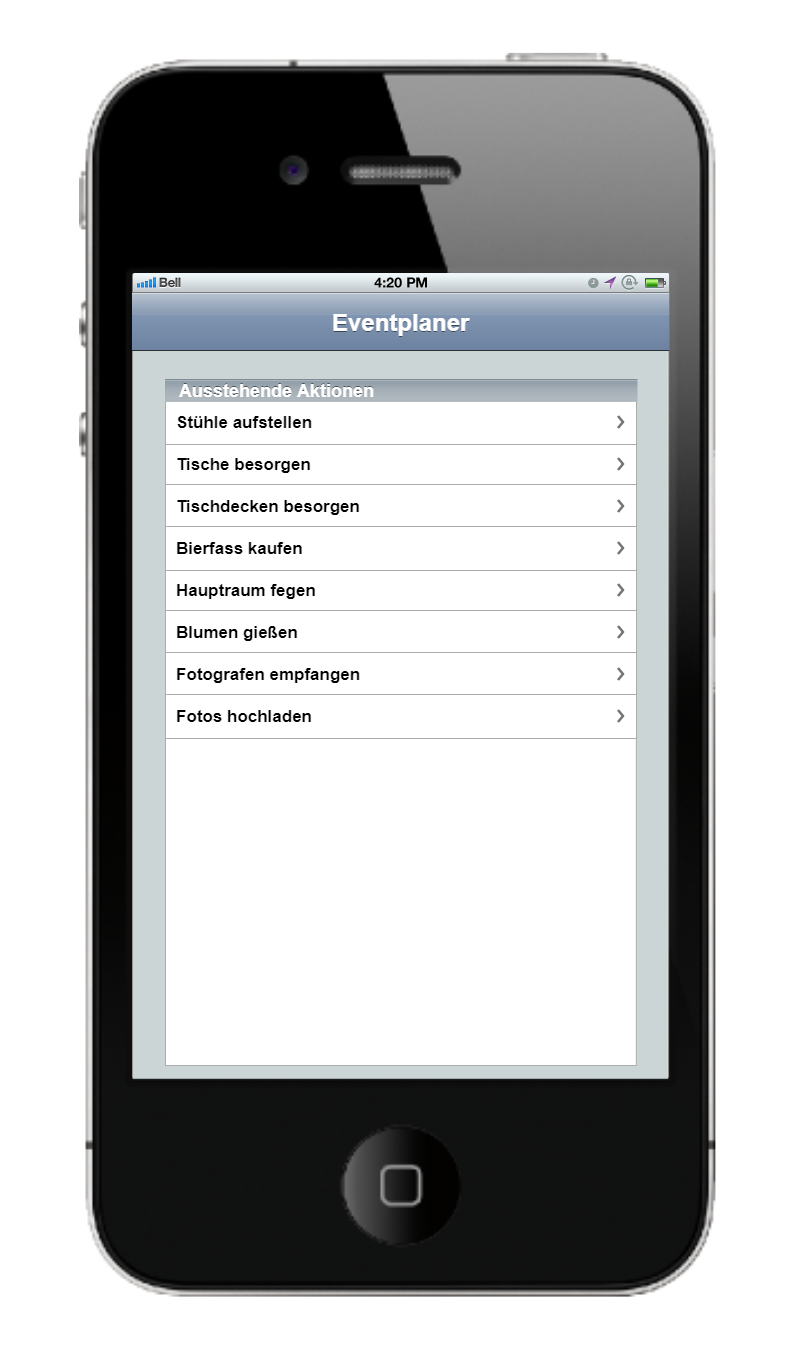
\includegraphics[width=0.4\columnwidth]{Bilder/mockup_mobile_overview.png}
    \caption{Einstiegsansicht der mobilen Version des Eventplaners}
    \label{fig:mockup:mobile:overview}
\end{figure}

In \autoref{fig:mockup:mobile:overview} ist ein Mockup einer Übersichtsseite der geplanten Mobilanwendung zu sehen. Der Nutzer sieht ausschließlich die ihm zugeteilten, ausstehenden Aktionen und kann durch ein Tippen auf eine dieser Aktionen zu den Details gelangen. Hier haben wir darauf geachtet, dem Nutzer eine minimale Benutzeroberfläche zu bieten, um bei der Arbeit mit der Anwendung nicht durch komplizierte Menüs navigieren zu müssen, sondern nur Informationen zu sehen.

\begin{figure}[ht!]
    \centering
    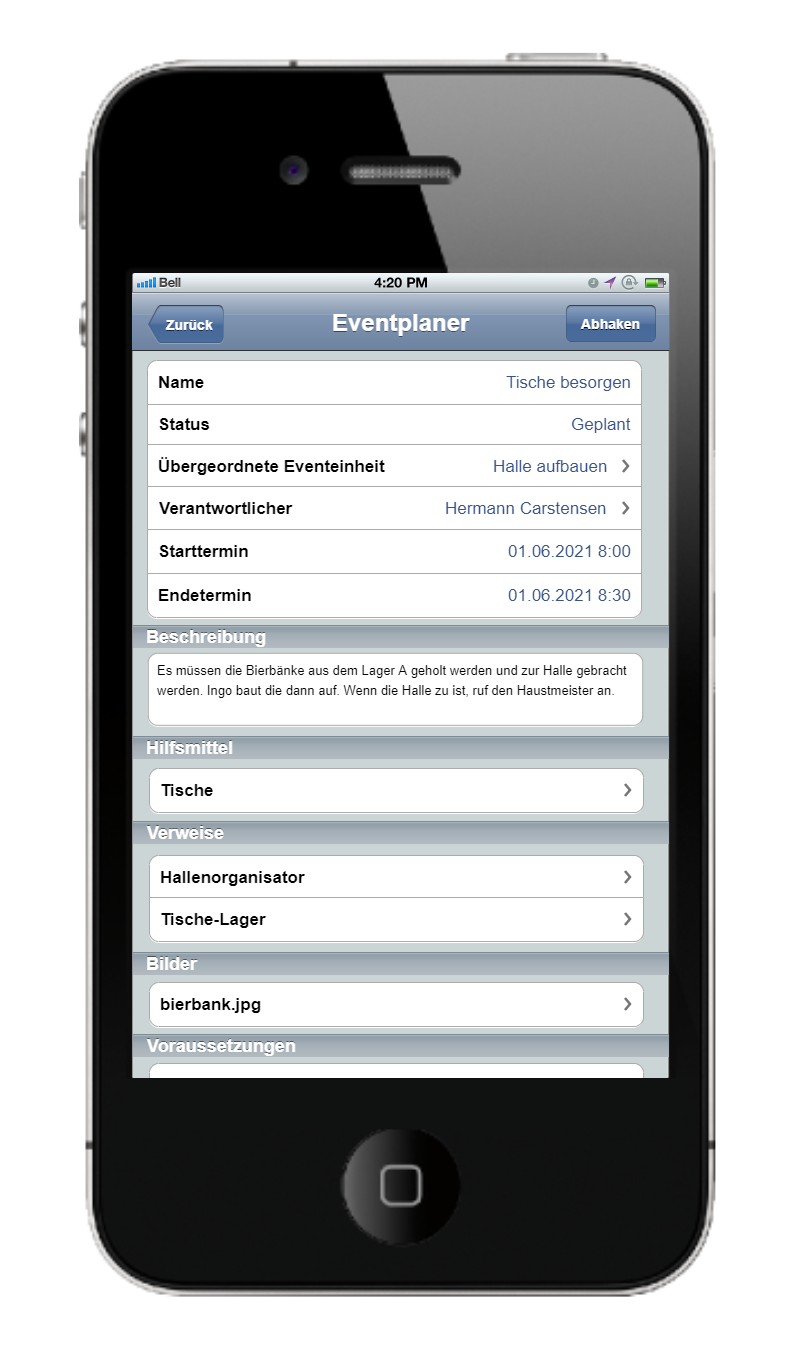
\includegraphics[width=0.4\columnwidth]{Bilder/mockup_mobile_object_page.png}
    \caption{Detailansicht einer Aktion der mobilen Version des Eventplaners}
    \label{fig:mockup:mobile:detail}
\end{figure}

In \autoref{fig:mockup:mobile:detail} ist das Mockup der Detailansicht einer Aktion in der mobilen Version des Eventplaners zu sehen. Hier ist ersichtlich, dass dem Nutzer alle notwendigen Informationen zur Verfügung stehen und jeweils durch ein Tippen auf zugeordnete Elemente wie Hilfsmittel, Verweise und den Verantwortlichen auf die Details dieser Objekte navigiert werden kann. Des Weiteren ist zu sehen, dass in der Kopfleiste der Anwendung zwei Knöpfe vorhanden sind: Links ein Zurück-Knopf, um wieder auf die Übersicht zu gelangen und rechts ein Knopf mit der Aufschrift \enquote{Abhaken}. Durch diesen Knopf kann der Nutzer, da er der Hauptverantwortliche der geöffneten Teileinheit ist, diese Teileinheit in den Status \enquote{Fertig} versetzen.

Damit sind die Anforderungen des Kunden im Mockup der Mobilanwendung sowie durch die Schnittstelle realisierbar und können problemlos in der zweiten Ausbaustufe der Software umgesetzt werden.

\FloatBarrier
\section{Eventtemplates}

Das wesentliche Ziel unserer Software ist es, die Abläufe in den Unternehmen unserer Kunden zu unterstützen und effizienter zu gestalten. Hierzu gehört insbesondere die Vermeidung bzw. Automatisierung trivialer oder repetitiver Tätigkeiten. Gerade repetitive Aufgaben können bei der Eventplanung auftreten, wenn Events gleicher Art, wie beispielsweise mehrere Hochzeiten oder mehrere Kongresse, geplant werden müssen, da hier häufig ähnliche Abläufe und Teileinheiten auftreten. Um nun die Planung ähnlicher Abläufe nicht bei jedem Event händisch durchführen zu müssen, wünschte der Kunde die Möglichkeit, sogenannte Eventelemente verwenden zu können, welche als Vorlagen für Events oder Teileinheiten dienen können. Dieser Gedanke wurde von uns aufgegriffen und noch weiter verfeinert. So kennt unsere Software unter dem Oberbegriff \enquote{Eventtemplates} sowohl \enquote{Eventelemente}, als auch \enquote{Teilelemente}. Wie die Namen bereits vermuten lassen, dienen erstere als Vorlagen für ganze Events, letztere als Vorlagen für einzelne Teileinheiten. Eventelemente können hierbei analog zu Events beliebig viele Teilelemente beinhalten, welche wiederum als Vorlagen für einzelne Teileinheiten dienen. Im Zuge der Modellierung wurde von uns also der im Lastenheft verwendete grobe Begriff \enquote{Eventelemente} aufgebrochen und unterschieden in Vorlagen für Events und Vorlagen für Teileinheiten. Diese Unterscheidung ermöglicht es den Nutzern, spezifischere Vorlagen für bestimmte Anwendungen zu definieren und auf diese Weise bei deren Verwendung noch weniger immergleiche Tätigkeiten ausführen zu müssen.

\section{Gestaltung des Entwurfes mit Fokus auf Flexibilität in der Arbeitsweise}
Da bei der Analyse des Lastenheftes und dem damit einhergehenden Kontakt mit dem Kunden klar wurde, dass dieser möglichst viel Flexibilität beim Umgang mit der Software wünscht. Um dieser Anforderung gerecht zu werden, haben wir an vielen Stellen bewusst Freiheiten gelassen und schränken den Nutzer somit nicht unnötig ein.

Ein Beispiel hierfür ist, dass Mitarbeiter bei uns für mehrere sich überlappende Teileinheiten gleichzeitig verantwortlich sein können. So wird es erfahrenen Mitarbeitern ermöglicht, ihre Zeit zwischen den Aufgaben dynamisch aufzuteilen und der Kunde kann auf diese Weise deren Arbeitserfahrung und Zeitmanagementfähigkeiten optimal nutzen.

Ein weiteres Beispiel ist in der Verwendung vieler Freitextfelder zu sehen. Durch die Vorgabe einer festen Struktur bei Namen, Materialnummern oder Kategorie kann das Unternehmen seine organisatorischen Details ändern, ohne die Software anpassen zu müssen. Dieses Konzept ist auch bei den Verweisen zu sehen, denen Dokumente zugeordnet werden können. Die Software trifft keine Einschränkung in den Dateitypen der zuordenbaren Dokumente, sodass jede Datei einem Verweis zugeordnet werden kann. Dadurch benötigt der Nutzer keine weiteren Verzeichnisse und Anhänge zu Events, sondern kann alle Informationen zum Event direkt in der Software speichern.

Ein letztes Beispiel für diese Flexibilität ist in der Rollenzuweisung ersichtlich. Jeder Nutzer kann eine, mehrere oder alle Rollen besitzen. Dadurch ist gewährleistet, dass jede Verantwortlichkeit innerhalb des Unternehmens gut abgebildet werden kann, wie zum Beispiel ein Personalmitarbeiter, der gelegentlich auch als Montageleiter tätig ist.

Diese Beispiele zeigen, dass wir in unserem Entwurf großen Wert darauf gelegt haben, den Kunden nicht in seiner Arbeitsweise einzuschränken, sondern mit unserer Software zu unterstützen. Die vielen Möglichkeiten der Flexibilität zeigen eine Anpassungsfähigkeit der Software an die Prozesse des Unternehmens und verhindern somit dass kreative Ideen für Prozessoptimierungen an der Softwarekompatibilität scheitern.

\section{Desktoporientierte Benutzeroberfläche}
Um die Möglichkeiten eines Desktop-PCs bei der Darstellung mehrerer Fenster vollends auszunutzen, setzt unsere Software auf Wunsch des Kunden auf die Aufteilung verschiedener Aufgaben in verschiedene Fenster. So wird jede GUI zur Anzeige oder zur Bearbeitung eines Objektes in einem separaten Fenster angezeigt. Diese strukturierte Einteilung unterstützt den Endnutzer nicht nur dabei, die Übersicht über die von ihm Bearbeiteten Objekte mit ihren teilweise komplexen Zusammenhängen zu behalten, sondern ermöglicht es auch, mehrere Objekte zugleich zu öffnen. Dieses Feature ist besonders hilfreich, sollte der Nutzer beispielsweise beim Erstellen einer Teileinheit zusätzliche Informationen, etwa aus einer anderen Teileinheit oder dem übergeordneten Event, benötigen. Durch die Möglichkeit, mehrere Fenster parallel zu öffnen, kann er diese Informationen leicht erhalten, ohne seine eigentliche Arbeit zu unterbrechen und die dafür notwendige Ansicht zu verlassen, wie es bei einer Anwendung mit nur einem einzigen Fenster nötig wäre. Auf diese Weise unterstützt unsere Software aktiv den Workflow der Nutzer und steigert somit deren Produktivität und Motivation.

\section{Unterscheidung in Verbrauchsgut und Gebrauchsgut}
Bereits bei der Analyse des Lastenhefts wiesen wir in einer unserer Fragen darauf hin, dass es sinnvoll wäre, verschiedene Arten von Hilfsmitteln mit unterschiedlichen Attributen zu unterscheiden. Dieser Vorschlag wurde durch den Kunden angenommen und er beauftragte uns, bei der Modellierung der Hilfsmittel zwei verschiedene Arten derselben zu unterschieden: Zum einen die Gebrauchsgüter, welche mehrfach benutzt werden können und dabei der Abnutzung unterliegen, zum anderen die Verbrauchsgüter, welche nach einmaliger Nutzung verbraucht sind und dementsprechend nicht wiederverwendet werden können. 

Der wesentliche Unterschied bei der Verwaltung der beiden Arten von Hilfsmitteln liegt darin, dass für ein Verbrauchsgut lediglich die insgesamt verfügbare Menge gespeichert werden muss. Sobald eine gewisse Stückzahl des Verbrauchsgutes durch eine Verwendung für eine Aktion gebucht wird gilt diese als verbraucht und die im System hinterlegte Menge wird entsprechend reduziert. Aus diesem Grund muss für die schnell aufgebrauchten Verbrauchsgüter ein ständiger Nachschub gewährleistet werden. Um diesen Prozess zu unterstützen, bietet unser System die Möglichkeit, für jedes Verbrauchsgut einen Lieferanten zu hinterlegen. Auf diese Weise können bei knappem Lagerbestand Verbrauchsgüter ohne großen Suchaufwand nachbestellt werden. 

Das Hinterlegen eines Lieferanten ist bei den Gebrauchsgütern nicht notwendig und wurde darum auch nicht von uns umgesetzt, um die Software möglichst einfach und ohne überflüssige Funktionalitäten zu gestalten. Dafür erwies sich die Berechnung der für einen bestimmten Zeitraum verfügbaren Menge eines Gebrauchsgutes vergleichsweise komplex. Durch den Nutzer gepflegt werden muss dennoch lediglich die Gesamtmenge des Gebrauchsgutes, welche der Kunde besitzt. Möchte er nun ein Gebrauchsgut für einen bestimmten Zeitraum für eine Aktion buchen, so wird durch das System automatisch die für den geplanten Zeitraum verfügbare Menge auf Basis der vorhanden Gesamtmenge sowie weiterer Buchungen des Gebrauchsgutes berechnet. Auf diese Weise kann ein Mangel an einem bestimmten Gebrauchsgut frühzeitig erkannt und behoben werden. 

Diese Unterscheidung wurde von uns bereits bei der Entwicklung des Analyseklassendiagramms berücksichtigt und wird auch in der Implementierung umgesetzt werden. Da wir stets mit dem Ziel arbeiten, unsere Software für alle Beteiligten möglichst transparent zu gestalten und darum nach den Methoden des Domain-driven Design arbeiten, wurde selbstverständlich auch die durch den Kunden vorgeschlagene Nomenklatur für die beiden Arten von Hilfsmitteln von der Analyse bis hin zur Implementierung beibehalten. 
